\chapter{Theoretical Background} % <<< --------------------------------------- %
\label{ch:analog-to-digital_data_aquisition}
% ---------------------------------------------------------------------------- %

\section{Analog-to-Digital Data Acquisition}
\label{sec:adc-acquisition}

\subsection{The DSP Chain}
\label{subsec:dsp-chain}

Digitally acquiring a signal generally requires at least the following steps:

\begin{itemize}\tightlist
    \item
        Analog LP: Remove any frequencies above fs/2, to enable correct processing
        down the chain (more on this later).
    \item
        ADC: convert time-continuous and value-continuous into value-discreet and
        time-discreet signal. Being value-discreet is of less importance in our
        system, but let it be mentioned that this is the source of the quantization
        noise. Being time-discreet has a few more consequences:
        \begin{itemize}\tightlist
                \item
                    multiplication w/ dirac pulse sequence in time domain
                \item
                    convolution w/ dirac pulse sequence in frequency domain
                \item
                    spectrum of signal is repeated at intervals of fs, centered
                    around each multiple of fs.
                \item
                    if the signal has frequency components above fs/2, this means
                    that different copies of the signal's spectrum will overlap
                    and lead to an error called aliasing. This means that the
                    analog waveform can no longer be unambiguously reconstructed
                    and correct processing of the data down the chain is not possible.
                    The phenomenon called "folding back" is also a consequence of
                    this and will be described in more detail later, because it is
                    of particular importance for our system.
                \item
                    As a consequences, the analog low-pass filter is required.
        \end{itemize}
    \item
        DSP: Can be n inalmost arbitrary. Preferred to analog signal processing because
        it can be done with computers, which are well understood and cheap.
        Primary problem tends to be the amount of data being shoved into the DSP
        system, which is usually constrained with regards to its available resources
        (i.e. processing power). If the ADC provides too much data for the DSP to
        meaningfully process (keep in mind: depending on \emph{what} is to be done
        in the DSP part, sometimes the ADC's data rate might be too high, other times
        not, so it is usually not possible to perfectly match the ADC's specifications
        to the DSP unless the application's scope is very narrowly defined before the
        system is designed).
\end{itemize}

The solution to the problem of too much data is usually downsampling. One could run
the ADC at lower clock frequencies, but oversampling carries some advantages which would
be lost with that.

\subsection{Challenges in Downsampling}
\label{subsec:downsampling}

The most obvious way to downsample from a sequence of values is of course to simply pick
each nth sample. However, this has some serious drawbacks which make it an unworkable solution
in most cases.

\textbf{Fancy Graphics of downsampling without LP filter with explanations}


\subsection{Digital Low-Pass Filters}
\label{subsec:digital-lp-filters}

The obvious solution to this predicament is to apply a (digital) low-pass filter to the
sequence of values before downsampling. For this purpose, three types of filters are commonly
used, each with their own specific advantages and drawbacks: IIR, FIR, CIC.

For theseandthose reasons, we will use FIR and CIC in our system.

\textbf{Fancy graphics of LP filter, downsampling and folding back}

\section{Designing a Filter System}
\label{sec:designing-a-filter-system}

Talking about which type of filter has which properties is all good and well in theory, but
how does one actually apply this knowledge to a practical problem? This section answers that
question insofar as it applies to our project.

\begin{itemize}\tightlist
    \item
        limited HW resources
    \item
        single-stage vs. multi-stage
    \item
        TBW issue with multi-stage
    \item
        filters at lower frequencies use fewer resources
    \item
        halfband filtres
    \item
        CIC: compensation filters
\end{itemize}

\begin{figure}
    \centering
    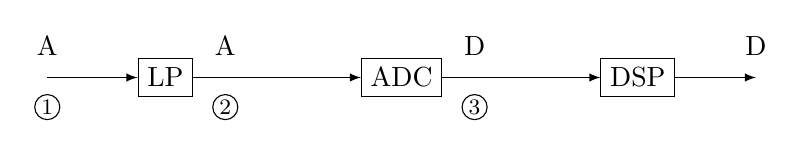
\begin{tikzpicture}
    \coordinate (in) at (-1.5,0);
    \coordinate (out) at (7.5,0);

    \node[draw] (LP)  at (0,0) {LP};
    \node[draw] (ADC) at (3,0) {ADC};
    \node[draw] (DSP) at (6,0) {DSP};

    \draw[-latex] (in)  -- (LP);
    \draw[-latex] (LP)  -- (ADC);
    \draw[-latex] (ADC) -- (DSP);
    \draw[-latex] (DSP) -- (out);

    \node[above      =1ex] (a1a) at (in)       {A};
    \node[above right=1ex] (a2a) at (LP.east)  {A};
    \node[above right=1ex] (d1a) at (ADC.east) {D};
    \node[above      =1ex] (d2a) at (out)      {D};

    \node[draw,circle,below=4ex,inner sep=0.30mm] (a1b) at (a1a) {\footnotesize 1};
    \node[draw,circle,below=4ex,inner sep=0.30mm] (a2b) at (a2a) {\footnotesize 2};
    \node[draw,circle,below=4ex,inner sep=0.30mm] (d1b) at (d1a) {\footnotesize 3};
\end{tikzpicture}

    \caption{Digital signal processing chain from analog signal to the digitally processed data stream}
    \label{fig:dspChain:blocks}
\end{figure}

\begin{figure}
    \centering
    \begin{tikzpicture}
     \pgfplotsset{every axis/.style={
            height=30mm,
            width=40mm,
            grid=none,
            axis line style={draw=none},
            tick style={draw=none},
            ticks = none,
        }
    }
    \begin{axis}[
        at = {(0,0)},
    ]
        \addplot[-]            table[x=t,y=y,col sep=comma] {images/dspChain/noisySine.csv};
    \end{axis}

    \begin{axis}[
        at = {(40mm,0)},
    ]
        \addplot[-,smooth]     table[x=t,y=y,col sep=comma] {images/dspChain/smoothSine.csv};
    \end{axis}

    \begin{axis}[
        at = {(80mm,0)},
    ]
        \addplot[ycomb,mark=o,mark size=1.0] table[x=t,y=y,col sep=comma] {images/dspChain/sampledSine.csv};
    \end{axis}
    \draw[-latex] (2.5,0.75) -- (3.85,0.75);
    \draw[-latex] (6.5,0.75) -- (7.85,0.75);

    \node[draw,inner sep=0.3mm,circle] at (1.25,1.75) {\footnotesize 1};
    \node[draw,inner sep=0.3mm,circle] at (5.25,1.75) {\footnotesize 2};
    \node[draw,inner sep=0.3mm,circle] at (9.25,1.75) {\footnotesize 3};
\end{tikzpicture}

    \caption{Digital signal processing chain from analog signal to the digitally processed data stream}
    \label{fig:dspChain:timedomain}
\end{figure}

\begin{figure}
    \centering
    \tikzsetnextfilename{dspChainFreqDomain}
\begin{tikzpicture}
     \pgfplotsset{every axis/.style={
            height=25mm,
            width=30mm,
            grid=none,
            axis line style={draw=none},
            tick style={draw=none},
            ticks = none,
        }
    }
    \begin{axis}[
        at = {(0,0)},
    ]
        \addplot[thick,q1,-]
            table[x=t,y=y,col sep=comma] {images/dspChain/spectrumFlat.csv};
    \end{axis}

    \begin{axis}[
        at = {(40mm,0)},
    ]
        \addplot[thick,q1,-,smooth]
            table[x=t,y=y,col sep=comma] {images/dspChain/spectrumLP.csv};
    \end{axis}

    \begin{axis}[
        at = {(80mm,0)},
    ]
        \addplot[thick,q1,-,smooth]
            table[x=t,y=y,col sep=comma] {images/dspChain/spectrumSampled.csv};
    \end{axis}
    \draw[-latex] (2.9,1.25) -- (3.95,1.25);
    \draw[-latex] (6.9,1.25) -- (7.95,1.25);

    %\node[draw,inner sep=0.3mm,circle] at (1.25,1.75) {\footnotesize 1};
    %\node[draw,inner sep=0.3mm,circle] at (5.25,1.75) {\footnotesize 2};
    %\node[draw,inner sep=0.3mm,circle] at (9.25,1.75) {\footnotesize 3};
\end{tikzpicture}

    \caption{Digital signal processing chain from analog signal to the digitally processed data stream}
    \label{fig:dspChain:freqDomain}
\end{figure}

\begin{figure}
    \centering
    \begin{tikzpicture}
     \pgfplotsset{every axis/.style={
            height=40mm,
            width=120mm,
            grid=none,
            axis line style={draw=none},
            tick style={draw=none},
            ticks = none,
        }
    }
    \begin{axis}[
        at = {(0mm,30mm)},
    ]
        \addplot[-]            table[x=f,y=Y,col sep=comma] {images/aliasing/bandNoAliasing.csv};
    \end{axis}

    \begin{axis}[
        at = {(0mm,0mm)},
    ]
        \addplot[-]            table[x=f,y=Y,col sep=comma] {images/aliasing/bandAliased1.csv};
        \addplot[-]            table[x=f,y=Y,col sep=comma] {images/aliasing/bandAliased2.csv};
        \addplot[-]            table[x=f,y=Y,col sep=comma] {images/aliasing/bandAliased3.csv};
    \end{axis}
\end{tikzpicture}

    \caption{Digital signal processing chain from analog signal to the digitally processed data stream}
    \label{fig:aliasing:band}
\end{figure}

\begin{figure}
    \centering
    \begin{tikzpicture}
     \pgfplotsset{every axis/.style={
            height=40mm,
            width=120mm,
            grid=none,
            axis line style={draw=none},
            tick style={draw=none},
            ticks = none,
        }
    }
    % fs = 4
    % fs/2 = 2
    
    % Dirac at f=1
    \begin{axis}[
        at = {(0mm,30mm)},
    ]
        % Centered around 0
        \addplot[ycomb,mark=triangle*] coordinates {
            (1,1)
            (-1,1)
        };
        % Centered around fs = 4
        \addplot[blue,ycomb,mark=triangle*] coordinates {
            (3,1)
            (5,1)
        };
        % Centered around -fs = -4
        \addplot[magenta,ycomb,mark=triangle*] coordinates {
            (-3,1)
            (-5,1)
        };
    \end{axis}

    % Dirac at f=3
    \begin{axis}[
        at = {(0mm,0mm)},
    ]
        % Centered around 0
        \addplot[ycomb,mark=triangle*] coordinates {
            (3,1)
            (-3,1)
        };
        % Centered around fs = 4
        \addplot[blue,ycomb,mark=triangle*] coordinates {
            (1,1)
            (7,1)
        };
        % Centered around -fs = -4
        \addplot[magenta,ycomb,mark=triangle*] coordinates {
            (-1,1)
            (-7,1)
        };
    \end{axis}
\end{tikzpicture}

    \caption{Digital signal processing chain from analog signal to the digitally processed data stream}
    \label{fig:aliasing:dirac}
\end{figure}

\begin{figure}
    \centering
    \tikzsetnextfilename{firTopology}
% https://tex.stackexchange.com/a/183092/131649
\begin{tikzpicture}[
    triangle/.style = {draw,regular polygon, regular polygon sides=3 },
    node rotated/.style = {rotate=180},
    border rotated/.style = {shape border rotate=180}
]    
    \coordinate (in) at   (0,0);
    \coordinate (out) at (12,-2);

    % Delay elements
    \node[draw] (d1) at  (2,0) {$z^{-1}$};
    \node[draw] (d2) at  (4,0) {$z^{-1}$};
    \node[draw] (d3) at  (6,0) {$z^{-1}$};
    \node       (d4) at  (8,0) {\ldots};
    \node[draw] (d5) at (10,0) {$z^{-1}$};

    % Multipliers
    \node[triangle, border rotated] (m1) at  (1,-1) {};
    \node[triangle, border rotated] (m2) at  (3,-1) {};
    \node[triangle, border rotated] (m3) at  (5,-1) {};
    \node[triangle, border rotated] (m4) at  (7,-1) {};
    \node[triangle, border rotated] (m5) at (11,-1) {};

    % Adders
    \node[draw,circle, inner sep=0.3mm] (a1) at  (3,-2) {$+$};
    \node[draw,circle, inner sep=0.3mm] (a2) at  (5,-2) {$+$};
    \node[draw,circle, inner sep=0.3mm] (a3) at  (7,-2) {$+$};
    \node                               (a4) at  (9,-2) {\ldots};
    \node[draw,circle, inner sep=0.3mm] (a5) at (11,-2) {$+$};

    % Lines
    \draw[-latex] (in) -- (d1);
    \draw[-latex] (in) -| (m1);
    \draw[-latex] (d1) -- (d2);
    \draw[-latex] (d1) -| (m2);
    \draw[-latex] (d2) -- (d3);
    \draw[-latex] (d2) -| (m3);
    \draw[-latex] (d3) -- (d4);
    \draw[-latex] (d3) -| (m4);
    \draw[-latex] (d4) -- (d5);
    \draw[-latex] (d5) -| (m5);
    \draw[-latex] (m1) |- (a1);
    \draw[-latex] (m2) -- (a1);
    \draw[-latex] (a1) -- (a2);
    \draw[-latex] (m3) -- (a2);
    \draw[-latex] (a2) -- (a3);
    \draw[-latex] (m4) -- (a3);
    \draw[-latex] (a3) -- (a4);
    \draw[-latex] (a4) -- (a5);
    \draw[-latex] (m5) -- (a5);
    \draw[-latex] (a5) -- (out);
\end{tikzpicture}

    \caption{Digital signal processing chain from analog signal to the digitally processed data stream}
    \label{fig:filtertopologies:fir}
\end{figure}

\begin{figure}
    \centering
    \tikzsetnextfilename{iirTopology}
% https://tex.stackexchange.com/a/183092/131649
\begin{tikzpicture}[
    triangle/.style = {draw,regular polygon, regular polygon sides=3 },
    node rotated/.style   = {rotate=180},
    border rotatedA/.style = {shape border rotate=-90},
    border rotatedB/.style = {shape border rotate=90},
]    
    \coordinate (in)  at (0,0);
    \coordinate (out) at (8,0);

    % Delay elements
    \node[draw] (d1) at  (2,-1) {$z^{-1}$};
    \node[draw] (d2) at  (2,-3) {$z^{-1}$};
    \node[draw] (d3) at  (6,-1) {$z^{-1}$};
    \node[draw] (d4) at  (6,-3) {$z^{-1}$};

    % Multipliers
    \node[triangle, border rotatedA] (m1) at  (3,0) {};
    \node[triangle, border rotatedA] (m2) at  (3,-2) {};
    \node[triangle, border rotatedA] (m3) at  (3,-4) {};
    \node[triangle, border rotatedA] (m4) at  (5,0) {};
    \node[triangle, border rotatedB] (m5) at  (5,-2) {};
    \node[triangle, border rotatedB] (m6) at  (5,-4) {};

    %% Adders
    \node[draw,circle, inner sep=0.3mm] (a1) at  (4,0) {$+$};
    \node[draw,circle, inner sep=0.3mm] (a2) at  (4,-2) {$+$};
    \node[draw,circle, inner sep=0.3mm] (a3) at  (4,-4) {$+$};

    %% Lines
    \draw[-latex] (in) -- (m1);
    \draw[-latex] (in) -| (d1);
    \draw[-latex] (d1) -- (d2);
    \draw[-latex] (d1) |- (m2);
    \draw[-latex] (d2) |- (m3);
    \draw[-latex] (m1) -- (a1);
    \draw[-latex] (m2) -- (a2);
    \draw[-latex] (m3) -- (a3);
    \draw[-latex] (a1) -- (m4);
    \draw[-latex] (m5) -- (a2);
    \draw[-latex] (m6) -- (a3);
    \draw[-latex] (d3) |- (m5);
    \draw[-latex] (d3) -- (d4);
    \draw[-latex] (d4) |- (m6);
    \draw[-latex] (m4) -| (d3);
    \draw[-latex] (m4) -- (out);
\end{tikzpicture}

    \caption{Digital signal processing chain from analog signal to the digitally processed data stream}
    \label{fig:filtertopologies:iir}
\end{figure}

\begin{figure}
    \centering
    %\tikzsetnextfilename{cicTopology}
% https://tex.stackexchange.com/a/183092/131649
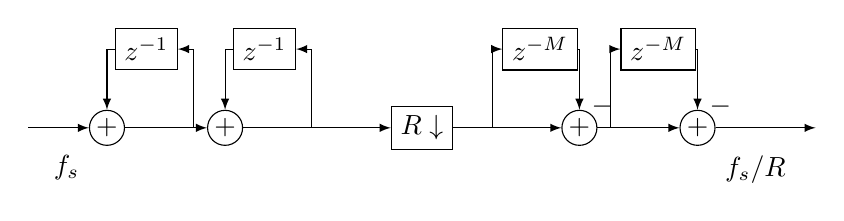
\begin{tikzpicture}
    \coordinate (in)  at  (0,0);
    \coordinate (out) at (10,0);

    % branching coordinates
    \coordinate (b1) at (2.1,0); % delta: 1.5
    \coordinate (b2) at (3.6,0); % delta: 1.5
    \coordinate (b3) at (5.9,0); % delta: 1.8
    \coordinate (b4) at (7.4,0); % delta: 1.5

    % Delay elements
    \node[draw] (d1) at  (1.5,1) {$z^{-1}$};
    \node[draw] (d2) at  (3.0,1) {$z^{-1}$};
    \node[draw] (d3) at  (6.5,1) {$z^{-M}$};
    \node[draw] (d4) at  (8.0,1) {$z^{-M}$};

    % Downsampler
    \node[draw] (r1) at (5,0) {$R\downarrow$};

    % Adders
    \node[draw,circle, inner sep=0.3mm] (a1) at  (1.0,0) {$+$};
    \node[draw,circle, inner sep=0.3mm] (a2) at  (2.5,0) {$+$};
    \node[draw,circle, inner sep=0.3mm] (a3) at  (7.0,0) {$+$};
    \node[draw,circle, inner sep=0.3mm] (a4) at  (8.5,0) {$+$};

    % subtractors
    \node[above right=0.2ex] (s1) at (a3) {$-$};
    \node[above right=0.2ex] (s2) at (a4) {$-$};

    % Lines
    \draw[-latex] (in) -- (a1);
    \draw[-latex] (a4) -- (out);
    \draw[-latex] (b1) |- (d1);
    \draw[-latex] (b2) |- (d2);
    \draw[-latex] (a1) -- (a2);
    \draw[-latex] (a2) -- (r1);
    \draw[-latex] (r1) -- (a3);
    \draw[-latex] (a3) -- (a4);
    \draw[-latex] (d1) -| (a1);
    \draw[-latex] (d2) -| (a2);
    \draw[-latex] (b3) |- (d3);
    \draw[-latex] (b4) |- (d4);
    \draw[-latex] (d3) -| (a3);
    \draw[-latex] (d4) -| (a4);

    % Annotations
    \node[below left =1.5ex] at (a1) {$f_s$};
    \node[below right=1.5ex] at (a4) {$f_s/R$};
\end{tikzpicture}

    \caption{Digital signal processing chain from analog signal to the digitally processed data stream}
    \label{fig:filtertopologies:cic}
\end{figure}

%>>>

%^^A vim: foldenable foldcolumn=4 foldmethod=marker foldmarker=<<<,>>>
